\chapter{2012 - PHYSICS 2A ACTUAL PRACTICAL A}

\begin{enumerate}
\item[1.] You are provided with a measuring cylinder, eureka can, nylon thread, standard masses and water. Proceed as follows:
\begin{enumerate}
\item[(a)] Pour water into eureka can until it is just beginning to overflow.

\begin{center}
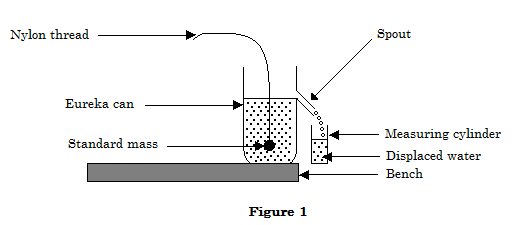
\includegraphics[width=13cm]{./img/2012-1-alt.png}
\end{center}

\item[(b)] Hold a suitable measuring cylinder under the spout and immerse a standard mass of 50 g into eureka can as shown in Figure 1. Water will pass through the spout and will be collected by the measuring cylinder. Wait for it to drop until it starts to cease and take long interval to drop. Record the reading of the water collected.
\item[(c)] Repeat the procedures in 1 (b) for standard masses of 100 g, 150 g, 200 g and 250 g.
\item[(d)] Tabulate your results showing the quantities as follows:\\

\begin{tabular}{|p{4cm}|p{4cm}|p{4cm}|}\hline
Mass (g) & Volume (cm$^3$) & Mass $\div$ Volume (g/cm$^3$) \\ \hline
50 & & \\ \hline
100 & & \\ \hline
150 & & \\ \hline
200 & & \\ \hline
250 & & \\ \hline
\end{tabular}\\[10pt]

\item[(e)] Plot a graph of mass against volume.
\item[(f)] State the nature of the graph.
\item[(g)] From the graph:
\begin{enumerate}
\item[(i)] Calculate the slope.
\item[(ii)] What does the slope of the graph show?
\item[(iii)] What is the relationship between mass and volume?
\item[(iv)] Establish the formula governing the experiment.
\end{enumerate}
\item[(h)] Identify with reasons the best to the least satisfactory method of finding the constant value of mass divide by volume.
\item[(i)] State two possible errors in this experiment.
\item[(j)] How can you minimize errors in 1 (i)?
\end{enumerate}

\pagebreak

\item[2.] You are provided with two plane mirrors, an optical pin, a sheet of plane drawing paper, mirror holder or office pins, a protractor, a ruler and a drawing table. Proceed as follows:
\begin{enumerate}
\item[(a)] Draw two lines at right angles.
\item[(b)] Place the two plane mirrors along the top two lines using the mirror holders or office pins as shown in Figure 2.

\begin{center}
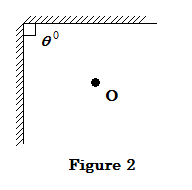
\includegraphics[width=5cm]{./img/2012-2-alt.png}
\end{center}

\item[(c)] Put an optical pin at O when $\theta = 90^\circ$. Look onto one of the mirrors and count the number of images, $n$, you see.
\item[(d)] Repeat the procedures in 2 (c) for $\theta = 72^\circ$, $\theta = 60^\circ$, $\theta = 45^\circ$ and $\theta = 30^\circ$.
\item[(e)] Tabulate your results for the values of $\theta$, $n$ and $\cfrac{360^\circ}{\theta}$.
\item[(f)] Plot a graph of number of images, $n$, against $\cfrac{360^\circ}{\theta}$.
\item[(g)] From the graph:
\begin{enumerate}
\item[(i)] Determine the slope.
\item[(ii)] Find the number of images when $\cfrac{360^\circ}{\theta} = 9$
\item[(iii)] Find the value of the $y$-intercept.
\item[(iv)] Derive the equation relating the number of images and $\cfrac{360^\circ}{\theta}$
\end{enumerate}
\item[(h)] From your experiment:
\begin{enumerate}
\item[(i)] What happens to the number of images as the value angle $\theta$ is reduced?
\item[(ii)] What happens to the number of images when $\theta = 0^\circ$?
\end{enumerate}
\item[(i)] State a possible source of error and how you can minimize it.
\item[(j)] What is the aim of this experiment?
\end{enumerate}
\end{enumerate}